%%%%%%%%%%%%%%%%%%%%%%%%%%%%%%%
%   Operazioni sugli Autori   %
%%%%%%%%%%%%%%%%%%%%%%%%%%%%%%%
\section{Operazioni sugli Autori}

%%%%%%%%%%%%%%%%%%%%%%%%%%%%%%
%     Visualizza Autore      %
%%%%%%%%%%%%%%%%%%%%%%%%%%%%%%
\subsection{Visualizzazione}
\begin{itemize}
	\item \textbf{Operazione}: ModificaAutore (con parametro operazione = 0)
	\item \textbf{Obiettivo}: Visualizza le informazioni relative ad un Autore presente nel database
	\item \textbf{Parametri}:
	\begin{enumerate}
		\item \textbf{idSessione}: in (da definire)
		\item \textbf{authorID}: in number
		\item \textbf{operazione}: in number
		\item \textbf{caller}: in varchar2 (nome della procedura chiamante, per redirect)
		\item \textbf{callerParams}: in varchar2 (parametri del chiamante)
	\end{enumerate}
	\item \textbf{Risultato}: Visualizza i dati relativi all'autore identificato da AuthorID, se presente nel database, restituisce un errore altrimenti
	\item \textbf{Errori}: 
	\begin{itemize}
		\item L'Autore identificato da AuthorID non è presente nel database
	\end{itemize}
	\item \textbf{Usa}: Autori
	\item \textbf{Modifica}: nessuno
	\item \textbf{Precondizioni}:
	\begin{itemize}
		\item $\exists x \in Autori : x.IdAutore = AuthorID$
	\end{itemize}
	\item \textbf{Postcondizioni}: nessuna
	\item \textbf{Note}: Oltre ai dettagli dell'autore è presente un form che permette di 
	visualizzare alcune statistiche relative all'autore:  \hyperref[OpereRealizzate]{\textbf{Opere realizzate}}, 
	\hyperref[MuseiOpereEsposte]{\textbf{Musei con opere esposte}},
	\hyperref[Collaborazioni]{\textbf{Collaborazioni effettuate}}.
\end{itemize}

%%%%%%%%%%%%%%%%%%%%%%%%%%%%%%
%      Inserisci Autore      %
%%%%%%%%%%%%%%%%%%%%%%%%%%%%%%
\subsection{Inserimento}
\begin{itemize}
	\item \textbf{Procedure coinvolte}: InserisciAutore, ConfermaDatiAutore, InserisciDatiAutore
	\item \textbf{Obiettivo}: Inserisce un nuovo autore nel database
	\item \textbf{Parametri}:
	\begin{enumerate}
		\item \textbf{authName}: in varchar2
		\item \textbf{authSurname}: in varchar2
		\item \textbf{dataNascita}: in date
		\item \textbf{dataMorte}: in date
		\item \textbf{nation}: in varchar2
	\end{enumerate}
	\item \textbf{Risultato}: Inserisce un nuovo autore nella tabella Autori con i dati specificati dai parametri, se consentito
	\item \textbf{Errori}: 
	\begin{itemize}
		\item È già presente nel database un autore con gli stessi dati
		\item La data di nascita dell'autore è posteriore alla data di morte
	\end{itemize}
	\item \textbf{Usa}: Autori
	\item \textbf{Modifica}: Autori
	\item \textbf{Precondizioni}:
	\begin{itemize}
		\item $authName \ne null \land authSurname \ne null \land nation \ne null$
		\item $dataNascita = null \\
		\lor dataMorte = null \\ 
		\lor (dataNascita \ne null \land dataMorte \ne null \land dataNascita < dataMorte)$
		\item $\nexists x \in Autori : x.Nome = authName \land x.Cognome = authSurname \\
		\land x.DataNascita = dataNascita \land x.DataMorte = dataMorte \\
		\land x.Nazionalita = nation$
		\item $|Autori| = n$
	\end{itemize}
	\item \textbf{Postcondizioni}:
	\begin{itemize}
		\item $(IdAutore,authName,authSurname,dataNascita,dataMorte,nation) \in Autori$
		\item $|Autori| = n + 1$
	\end{itemize}
\end{itemize}

%%%%%%%%%%%%%%%%%%%%%%%%%%%%%%
%      Modifica Autore      %
%%%%%%%%%%%%%%%%%%%%%%%%%%%%%%
\subsection{Modifica}
\begin{itemize}
	\item \textbf{Procedure coinvolte}: ModificaAutore (con parametro operazione = 1), UpdateAutore
	\item \textbf{Obiettivo}: Modifica i dati di un Autore presente nel database
	\item \textbf{Parametri}:
	\begin{enumerate}
		\item \textbf{authorID}: in number
		\item \textbf{operazione}: in number
		\item \textbf{caller}: in varchar2 (nome della procedura chiamante, per redirect)
		\item \textbf{callerParams}: in varchar2 (parametri del chiamante)
	\end{enumerate}
	\item \textbf{Risultato}: Modifica i dati di un Autore nella base di dati, oppure restituisce un errore (e non modifica la base di dati)
	\item \textbf{Errori}: 
	\begin{itemize}
		\item L'autore da modificare non è presente nella base di dati
		\item Data nascita posteriore alla data di morte (se specificate entrambe)
	\end{itemize}
	\item \textbf{Usa}: Autori
	\item \textbf{Modifica}: Autori
	\item \textbf{Precondizioni}:
	\begin{itemize}
		\item $\exists x \in Autori : x.IdAutore = AuthorID$
		\item $|Autori| = n$
	\end{itemize}
	\item \textbf{Postcondizioni}: $x \in Autori : x.IdAutore = AuthorID$ \\
	(i nuovi valori sono acquisiti e controllati tramite un form)
	\begin{itemize}
		\item $x.Nome := newName$
		\item $x.Cognome := newsurname$
		\item $x.DataNascita := newbirth$
		\item $x.DataMorte := newdeath$
		\item $x.Nazionalita := newnation$
		\item $|Autori| = n$
	\end{itemize}
\end{itemize}

%%%%%%%%%%%%%%%%%%%%%%%%%%%%%%
%       Elimina Autore       %
%%%%%%%%%%%%%%%%%%%%%%%%%%%%%%
\subsection{Eliminazione}
\begin{itemize}
	\item \textbf{Procedire coinvolte}: EliminazioneAutore, SetAutoreEliminato
	\item \textbf{Obiettivo}: Setta un Autore presente nel database a eliminato
	\item \textbf{Parametri}:
	\begin{enumerate}
		\item \textbf{AuthorID}: in number
	\end{enumerate}
	\item \textbf{Risultato}: Setta l'autore come eliminato, spostandolo dal menuAutori al menuAutoriEliminati
	\item \textbf{Errori}: 
	\begin{itemize}
		\item L'autore è già stato eliminato
	\end{itemize}
	\item \textbf{Usa}: Autori
	\item \textbf{Modifica}: Autori
	\item \textbf{Precondizioni}:
	\begin{itemize}
		\item $\exists x \in Autori : x.IdAutore = AuthorID \land x.Eliminato = 0$
		\item $|Autori| = n$
	\end{itemize}
	\item \textbf{Postcondizioni}:
	\begin{itemize}
		\item $\exists x \in Autori : x.IdAutore = AuthorID \land x.Eliminato = 1$
		\item $|Autori| = n$
	\end{itemize}
\end{itemize}


%%%%%%%%%%%%%%%%%%%%%%%%%%%%%%
%       Rimuovi Autore       %
%%%%%%%%%%%%%%%%%%%%%%%%%%%%%%
\subsection{Rimozione}
\begin{itemize}
	\item \textbf{Operazione}: RimozioneAutore, DeleteAutore
	\item \textbf{Obiettivo}: Rimuove un Autore dal database, se presente
	\item \textbf{Parametri}:
	\begin{enumerate}
		\item \textbf{AuthorID}: in number
	\end{enumerate}
	\item \textbf{Risultato}: Rimuove un Autore dalla base di dati, oppure restituisce un errore (e non modifica la base di dati)
	\item \textbf{Errori}: 
	\begin{itemize}
		\item L'autore da rimuovere ha delle Opere nella base di dati
	\end{itemize}
	\item \textbf{Usa}: Autori
	\item \textbf{Modifica}: Autori
	\item \textbf{Precondizioni}:
	\begin{itemize}
		\item $\exists x \in Autori : x.IdAutore = AuthorID$
		\item $\nexists x \in AutoriOpere : x.IdAutore = AuthorID$
		\item $|Autori| = n$
	\end{itemize}
	\item \textbf{Postcondizioni}:
	\begin{itemize}
		\item $\nexists x \in Autori : x.IdAutore = AuthorID$
		\item $|Autori| = n - 1$
	\end{itemize}
\end{itemize}


\subsection{Statistiche e monitoraggio}
La scelta dell'operazione di statistica o monitoraggio avviene tramite dei radiobutton in un popup raggiungibile dal menu autori.\\
A seconda della statistica scelta verranno presentati dei form per la selezione di un museo e/o di un autore su cui effettuare la statistica.\\
Il parametro passato dal radiobutton è operazione, con valori tra 0 e 5, che identifica nelle procedure chiamate la particolare statistica

%%%%%%%%%%%%%%%%%%%%%%%%%%%%%%%%%%%%%%%%%%%%%%%%%%%%%%%%%%%%%%%%%
%       Opere realizzate dall'Autore (in qualunque museo)       %
%%%%%%%%%%%%%%%%%%%%%%%%%%%%%%%%%%%%%%%%%%%%%%%%%%%%%%%%%%%%%%%%%
\subsubsection{Opere realizzate dall’Autore}
\label{OpereRealizzate}
\begin{itemize}
	\item \textbf{Procedure coinvolte}: SelezioneOpStatAut, SelezioneAutoreStatistica, StatisticheAutori
	\item \textbf{Obiettivo}: Visualizza la lista di opere realizzate dall'autore selezionato, suddivise per museo di appartenenza
	\item \textbf{Parametri}:
	\begin{enumerate}
		\item \textbf{operazione}: in number
		\item \textbf{authID}: in number
	\end{enumerate}
	\item \textbf{Risultato}: Stampa una pagina contenente tutte le opere realizzate dall'autore considerato (anche nessuna)
	\item \textbf{Errori}: nessuno
	\item \textbf{Usa}: Autori, Opere, AutoriOpere, Musei
	\item \textbf{Modifica}: nessuna
	\item \textbf{Precondizioni}:
	\begin{itemize}
		\item $\exists x \in Autori : x.IdAutore = AuthorID$
		\item $operazione  = 0$
	\end{itemize}
	\item \textbf{Postcondizioni}: nessuna
\end{itemize}

%%%%%%%%%%%%%%%%%%%%%%%%%%%%%%%%%%%%%%%%%%%%%%%%%%%%%%%%%%%%%%%%%
%             Musei con opere dell'autore esposte               %
%%%%%%%%%%%%%%%%%%%%%%%%%%%%%%%%%%%%%%%%%%%%%%%%%%%%%%%%%%%%%%%%%
\subsubsection{Musei con Opere dell’Autore esposte}
\label{MuseiOpereEsposte}
\begin{itemize}
	\item \textbf{Procedure coinvolte}: SelezioneOpStatAut, SelezioneAutoreStatistica, StatisticheAutori
	\item \textbf{Obiettivo}: Visualizza i musei nei quali sono esposte al momento opere dell'autore; per ogni museo sono mostrati i titoli delle opere ivi contenute
	\item \textbf{Parametri}:
	\begin{enumerate}
		\item \textbf{operazione}: in number
		\item \textbf{authID}: in number
	\end{enumerate}
	\item \textbf{Risultato}: Stampa una pagina contenente tutti i musei nei quali sono in esposizione opere dell'autore
	\item \textbf{Errori}: nessuno
	\item \textbf{Usa}: Autori, Opere, AutoriOpere, Musei
	\item \textbf{Modifica}: nessuna
	\item \textbf{Precondizioni}:
	\begin{itemize}
		\item $\exists x \in Autori : x.IdAutore = AuthorID$
		\item $operazione  = 1$
	\end{itemize}
	\item \textbf{Postcondizioni}: nessuna
\end{itemize}
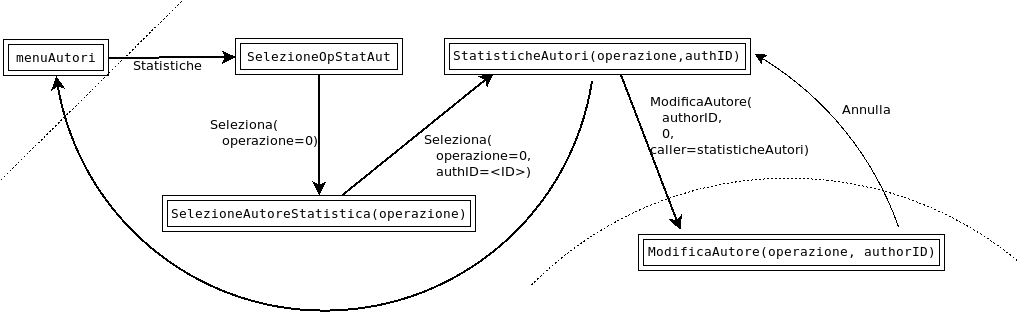
\includegraphics[width=\textwidth]{img/statAutori-0.png}\\[1cm]

\subsubsection{Collaborazioni effettuate}
\label{Collaborazioni}
\begin{itemize}
	\item \textbf{Procedure coinvolte}: SelezioneOpStatAut, SelezioneAutoreStatistica, StatisticheAutori
	\item \textbf{Obiettivo}: Visualizza le opere realizzate in collaborazione con altri autori presenti nella base di dati (anche nessuna)
	\item \textbf{Parametri}:
	\begin{enumerate}
		\item \textbf{operazione}: in number
		\item \textbf{authID}: in number
	\end{enumerate}
	\item \textbf{Risultato}: Stampa una pagina contenente tutte le opere realizzate dall'autore specificato ed un altro autore, raggruppandole per collaboratore
	\item \textbf{Errori}: nessuno
	\item \textbf{Usa}: Autori, Opere, AutoriOpere
	\item \textbf{Modifica}: nessuna
	\item \textbf{Precondizioni}:
	\begin{itemize}
		\item $\exists x \in Autori : x.IdAutore = AuthorID$
		\item $operazione  = 2$
	\end{itemize}
	\item \textbf{Postcondizioni}: nessuna
	\item \textbf{Note}: Poiché le opere sono raggruppate secondo il collaboratore
	è possibile che la stessa opera compaia più di una volta nella lista, sotto autori
	diversi
\end{itemize}
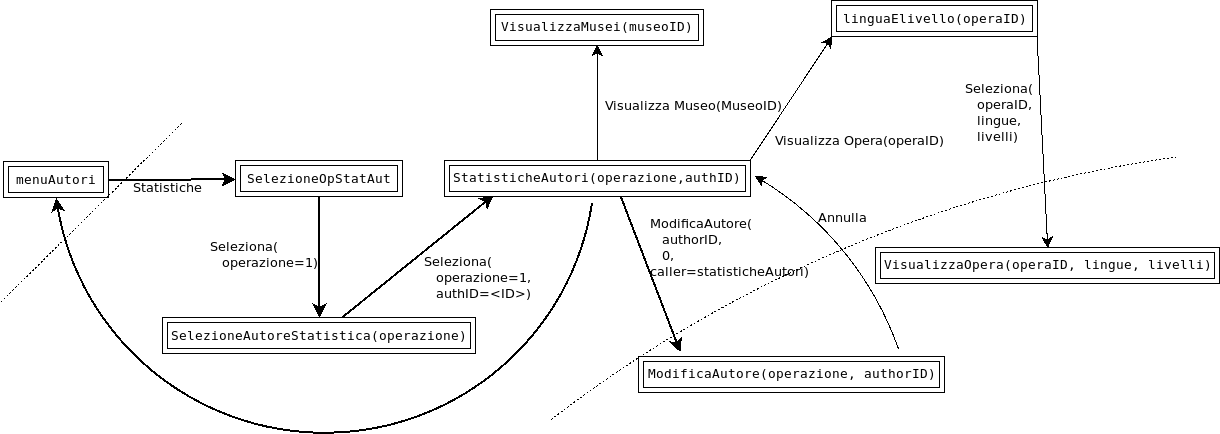
\includegraphics[width=\textwidth]{img/statAutori-1.png}\\[1cm]

\subsubsection{Opere dell’Autore presenti in un Museo scelto}
\begin{itemize}
	\item \textbf{Procedure coinvolte}: SelezioneOpStatAut, SelezioneAutoreStatistica, 
	StatisticheMuseoAutori
	\item \textbf{Obiettivo}: Visualizza le opere dell'autore specificato che sono esposte 
	nel museo scelto
	\item \textbf{Parametri}:
	\begin{enumerate}
		\item \textbf{operazione}: in number
		\item \textbf{authID}: in number
		\item \textbf{museoID}: in number
	\end{enumerate}
	\item \textbf{Risultato}: Stampa una pagina contenente tutte le opere realizzate dall'autore specificato che sono esposte all'interno del museo scelto
	\item \textbf{Errori}: nessuno
	\item \textbf{Usa}: Autori, Opere, AutoriOpere, Musei, SaleOpere, Stanze
	\item \textbf{Modifica}: nessuna
	\item \textbf{Precondizioni}:
	\begin{itemize}
		\item $\exists x \in Autori : x.IdAutore = AuthorID$
		\item $\exists y \in Musei : y.IdAutore = MuseoID$
		\item $operazione  = 3$
	\end{itemize}
	\item \textbf{Postcondizioni}: nessuna
\end{itemize}
%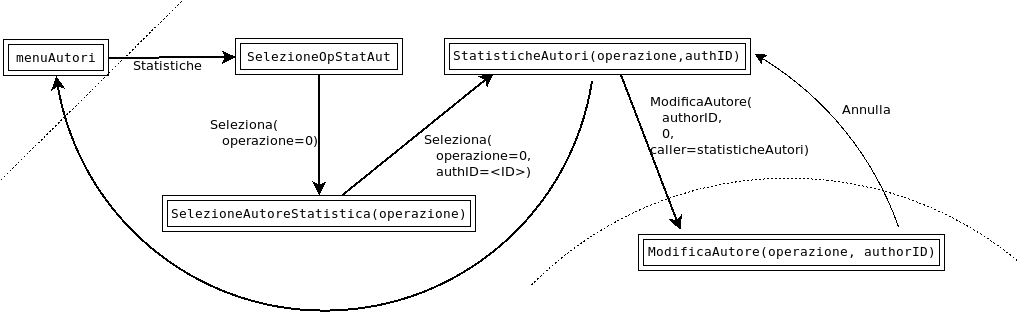
\includegraphics[width=\textwidth]{img/statAutori-0.png}\\[1cm]

\subsubsection{Autori in vita le cui Opere sono esposte in un Museo scelto}
\begin{itemize}
	\item \textbf{Procedure coinvolte}: SelezioneOpStatAut, SelezioneAutoreStatistica, 
	StatisticheMuseoAutori
	\item \textbf{Obiettivo}: Visualizza gli autori in vita (la cui data di morte è nulla)
	le cui opere sono esposte nel museo scelto
	\item \textbf{Parametri}:
	\begin{enumerate}
		\item \textbf{operazione}: in number
		\item \textbf{museoID}: in number
	\end{enumerate}
	\item \textbf{Risultato}: Stampa una pagina contenente tutti gli autori in vita
	 le cui opere sono esposte (potrebbero essere anche in prestito da un altro museo) 
	\item \textbf{Errori}: nessuno
	\item \textbf{Usa}: Autori, Opere, AutoriOpere, Musei, SaleOpere, Stanze
	\item \textbf{Modifica}: nessuna
	\item \textbf{Precondizioni}:
	\begin{itemize}
		\item $\exists y \in Musei : y.IdAutore = MuseoID$
		\item $operazione  = 4$
	\end{itemize}
	\item \textbf{Postcondizioni}: nessuna
	\item \textbf{Note}: Il parametro authID appare nell'URL nella pagina di 
	visualizzazione, ma soltanto con il valore di default: in realtà viene ignorato nella 
	logica dell'operazione
\end{itemize}

\subsubsection{Autori più prolifici (primi tre)}
\begin{itemize}
	\item \textbf{Procedure coinvolte}: SelezioneOpStatAut,SelezioneAutoreStatistica, classificaAutori
	\item \textbf{Obiettivo}: Visualizza i tre autori che hanno il maggior numero di opere
	all'interno della base di dati
	\item \textbf{Parametri}:
	\begin{enumerate}
		\item \textbf{operazione}: in number, in questo caso operazione=5
	\end{enumerate}
	\item \textbf{Risultato}: la lista dei tre autori che hanno realizzato più opere nella base di dati
	\item \textbf{Errori}: nessuno
	\item \textbf{Usa}: AutoriOpere, Autori
	\item \textbf{Modifica}: nessuno
	\item \textbf{Precondizioni}: nessuna
	\item \textbf{Postcondizioni}: nessuna
\end{itemize}